% !TeX TXS-program:compile = txs:///pdflatex/[--shell-escape]

\documentclass[9pt]{beamer}
\usetheme{Madrid}
\usecolortheme{beaver}
\usepackage{amsmath,amssymb,amsthm,asymptote,graphicx}
\usepackage{graphics}
% \usepackage{bisvslides}

\title{Counting}
\subtitle{Mathcounts 20 - Session 3}
\author{bisv.math@gmail.com}
\institute{BISV Mathcounts Club 20}
\date{December 2020}

%\maketitle
%~~~~~~~~~~~~~~~~~~~~~~~~~~~~~~~~~~~~~~~~~~~~~~~~~~~~~~~~~~~~~~~~~~~~~~~~~~~~~~
% Informations
%\title{TEMPLATE}

%\titlegraphic{assets/gkg.png} %change this to your preferred logo or image(the image is located on the top right corner).
%~~~~~~~~~~~~~~~~~~~~~~~~~~~~~~~~~~~~~~~~~~~~~~~~~~~~~~~~~~~~~~~~~~~~~~~~~~~~~~

\begin{document}

% Generate title page
\titlepage

% \begin{frame}

%  \frametitle{TABLE OF CONTENTS}
%  \tableofcontents
% \end{frame}


\section{Beginner Problems}
\begin{frame}
    \begin{alertblock}{}
        \begin{flushright}
        {\huge Beginner Problems}
        \end{flushright}
    \end{alertblock}
\end{frame}
%-----------------------------
% Difficulty: 1 • Answer: 2 faces
\begin{frame}[t]{5.1}
\begin{block}{}
    Jamie rolled a standard six-sided die that has each face painted either red, green or blue. In 100 rolls, the die landed with a red face up 50 times, with a blue face up 17 times, and with a green face up 33 times. Based on this data, how many faces of the die would you expect to be green?
\end{block}
\end{frame}

% Difficulty: 1 • Answer: 24
\begin{frame}[t]{5.2}
\begin{block}{}
  How many three-digit numbers greater than 700 can be formed using the digits 1, 3, 4, 7 and 9, if no repetition of digits is allowed in a number?
\end{block}
\end{frame}

% Difficulty: 2 • Answer: 44/125 
\begin{frame}[t]{5.3}
\begin{block}{}
 A large cube is dipped into red paint and then divided into 125 smaller congruent cubes. One of the smaller cubes is then randomly selected. What is the probability that the cube selected will have at least $25\%$ of its surface area painted red? Express your answer as a common fraction.
\end{block}
\end{frame}

% Difficulty: 2 • Answer: 5/9 
\begin{frame}[t]{5.4}
\begin{block}{}
    The nine regions on a spinner are numbered with positive integers 1 through 9, and the probability of the spinner landing on a given region is proportional to the label for that region. For example, since $4 \times 2 = 8$, the probability of landing on 8 is twice the probability of landing on 4. What is the probability that this spinner will land on an odd number? Express your answer as a common fraction.
\end{block}
\end{frame}

% Difficulty: 1 • Answer: 32 paths
\begin{frame}[t, fragile]{5.5}
\begin{block}{}
     Skipper follows a path along the grid shown, always moving either up or to the right. How many paths from $A$ to $C$ do not pass through $B$?
     
\end{block}
     \begin{center}
         \begin{asy}
         import cse5;
         //import olympiad;
         unitsize(1cm);
            draw((0,0)--(3,0), linewidth(2));
            draw((0,1)--(4,1), linewidth(2));
            draw((0,2)--(4,2), linewidth(2));
            draw((0,3)--(4,3), linewidth(2));
            draw((1,4)--(4,4), linewidth(2));
            draw((0,0)--(0,3), linewidth(2));
            draw((1,0)--(1,4), linewidth(2));
            draw((2,0)--(2,4), linewidth(2));
            draw((3,0)--(3,4), linewidth(2));
            draw((4,1)--(4,4), linewidth(2));
            filldraw(Circle((0,0),0.1));
            filldraw(Circle((2,2),0.1));
            filldraw(Circle((4,4),0.1));
            label("$A$", (0,0), SW);
            label("$B$", (2,2), NE);
            label("$C$", (4,4), NE);
         \end{asy}
     \end{center}

\end{frame}


% Difficulty: 2 • Answer: $\frac{1}{5}$ 
\begin{frame}[t]{5.6}
\begin{block}{}
     Six students (four juniors and two seniors) must be split into three pairs. If the pairs are chosen randomly, what is the probability that the two seniors form one pair? Express your answer as a common fraction.
\end{block}
\end{frame}

% Difficulty: 4 • Answer: 50 percent
\begin{frame}[t]{5.7}
\begin{block}{}
    Eighty percent of adults drink coffee and seventy percent drink tea. What is the smallest possible percent of adults who drink both coffee and tea?
\end{block}
\end{frame}

\newpage

\section{Intermediate Problems}
\begin{frame}
    \begin{alertblock}{}
        \begin{flushright}
        {\huge Intermediate Problems}
        \end{flushright}
    \end{alertblock}
\end{frame}

% Difficulty: 3 • Answer: 1/49
\begin{frame}[t]{6.1}
\begin{block}{}
     All of the possible sequences of four consecutive positive integers less than $200$ are created. One of these sequences is called orderly if the smallest member is divisible by $2$, the next smallest member is divisible by $3$, the next smallest is divisible by $4$, and the largest is divisible by $5.$ What is the probability that a randomly-selected sequence is orderly? Express your answer as a common fraction.
\end{block}
\end{frame}

% Difficulty: 4 • Answer: 12,441,600 orders 
% Product Rule
\begin{frame}[t]{6.2}
\begin{block}{}
    Mr. Reader has six different Spiderman comic books, five different Archie comic books and four different Garfield comic books. When stacked, all of the Spiderman comic books are grouped together, all of the Archie comic books are grouped together and all of the Garfield comic books are grouped together. In how many different orders can these 15 comic books be stacked in a pile with the covers facing up and all of them facing the same direction (that is, there is only one way to orient a book)? Express your answer as a whole number.
\end{block}
\end{frame}

% Difficulty: 4 • Answer: 36 elements
\begin{frame}[t]{6.3}
\begin{block}{}
    A subset $S$ of the set of integers from 50 to 100, inclusive, has the property that no two distinct elements of $S$ sum to 130. What is the maximum possible number of elements in $S$?
\end{block}
\end{frame}


% Difficulty: 4 • Answer: 35 arrangements
\begin{frame}[t, fragile]{6.4}
\begin{block}{}
    Matt will arrange four identical, dotless dominoes (shaded 1 by 2 rectangles) on the 5 by 4 grid below so that a path is formed from the upper left-hand corner $A$ to the lower righthand corner $B$. In a path, consecutive dominoes must touch at their sides and not just their corners. No domino may be placed diagonally; each domino covers exactly two of the unit squares shown on the grid. One arrangement is shown. How many distinct arrangements are possible, including the one shown?

\end{block}
\begin{center}
    \begin{asy}
        size(101);
        real w = 1; picture q;
        filldraw(q,(1/10,0)--(19/10,0)..(2,1/10)--(2,9/10)..(19/10,1)--(1/10,1)..(0,9/10)--(0,1/10)..cycle,gray(.6),linewidth(.6));
        add(shift(4*up)*q); add(shift(3*up)*shift(3*right)*rotate(90)*q); add(shift(1*up)*shift(3*right)*rotate(90)*q); add(shift(4*right)*rotate(90)*q);
        pair A = (0,5); pair B = (4,0);
        for(int i = 0; i<5; ++i)
        {draw((i,0)--(A+(i,0))); draw((0,i)--(B+(0,i)));}
        draw(A--(A+B));
        label("$A$",A,NW,fontsize(8pt)); label("$B$",B,SE,fontsize(8pt));
    \end{asy}
\end{center}
\end{frame}

% Difficulty: 4 • Answer: 372
\begin{frame}[t, fragile]{6.5}
\begin{block}{}
     How many routes are there to get from A to B if we can only travel to the right or up along the segments shown?
     
\end{block}
\begin{center}
    \begin{asy}
       unitsize(1cm);
       for(int i = 0; i<=8; ++i) {
           for(int j = 0; j<=5; ++j) {
               if(i<=7) {
                   if((!((j==2)||(j==3)))||((i==0)||(i>=4))) {
                       draw((i,j)--(i+1,j));
                   }
               }
               if(j<=4) {
                   if((i<=1)||(i>=4)){
                       draw((i,j)--(i,j+1));
                   }
               }
           }
       }
       draw((2,0)--(2,1));
       draw((2,4)--(2,5));
       label("A",(0,0),W);
       dot((0,0));
       label("B",(8,5),E);
       dot((8,5));
    \end{asy}
\end{center} 


\end{frame}

% Difficulty: 4 • Answer: 28
\begin{frame}[t]{6.6}
\begin{block}{}
    A number is called increasing if each of its digits is greater than the digit immediately to its left, if there is one. How many increasing numbers are there between $100$ and $200$?
\end{block}
\end{frame}

% Difficulty: 4 • Answer: 1/4
\begin{frame}[t]{6.7}
\begin{block}{}
    Four packages are delivered to four houses, one to each house. If these packages are randomly delivered, what is the probability that exactly two of them are delivered to the correct houses? Express your answer as a common fraction.
\end{block}
\end{frame}

\begin{frame}[t]{6.8}
\begin{block}{}
     How many subsets of one or more elements of the set {1, 2, 3, 4, 5, 6, 7, 8, 9, 10} contain the element 1 or the element 2 or both? \textit{Mathcounts Handbook 2020-21, \#236}
\end{block}
\end{frame}



\begin{frame}[t]{6.9}
\begin{block}{}
     Five fair coins are flipped. Those that land heads up are flipped again. After the second round of flips, what is the probability that all five coins are now tails up? Express your answer as a common fraction. \textit{Mathcounts Handbook 2020-21, \#228}
\end{block}
\end{frame}

\begin{frame}[t]{6.10}
\begin{block}{}
     The license plates in Eulerville are made of seven distinct characters, six of which are letters from A to Z inclusive and one of which is a digit from 0 to 9 inclusive. How many different Eulerville license plates include the word ``MATH'' with those four letters consecutive and in that order? \textit{Mathcounts Handbook 2020-21, \#212}
\end{block}
\end{frame}
%----------------------------
\newpage
\section{Challenge Problems}
\begin{frame}
    \begin{alertblock}{}
        \begin{flushright}
        {\huge Challenge Problems}
        \end{flushright}
    \end{alertblock}
\end{frame}
\begin{frame}[t]{7.1}
\begin{block}{}
     How many ways are there to arrange five red, five blue, and five green balls in a row so that no two green balls lie next to each other? \textit{(Russia)}
\end{block}
\end{frame}
% Difficulty: 5 • Answer: 126 permutations 
\begin{frame}[t]{7.2}
\begin{block}{}
     A sequence is $\textit{unimodal}$ if $a_1 < a_2 < \ldots < a_{k - 1} < a_k > a_{k + 1} > \ldots > a_{n - 1} > a_n$ for some value of $k$ such that $1 < k < n$. How many permutations of the numbers $1, 2, 3, 4, 5, 6, 7, 8$ form a unimodal sequence?
\end{block}
\end{frame}

\begin{frame}[t]{7.3}
\begin{block}{}
Two standard six-sided dice, each with faces numbered with the positive integers 1 through 6, have the probability distribution shown for the sum of the top-facing values on the dice. Two non-standard but fair six-sided dice can be numbered differently with nonnegative integers on each face and still yield the same probability distribution. Though a number may be on both dice, a number may not appear more than once on either die. If $a$ is the sum of the six numbers on one of these non-standard dice, and $b$ is the sum of the six numbers on the other die, what is the value of the product $a \times b$?
\textit{(MATHCOUNTS 2013-14 Handbook, \#269)}
\end{block}
% \begin{center}
    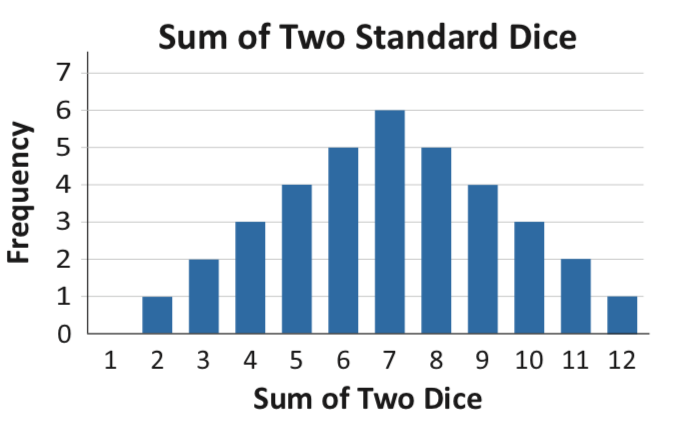
\includegraphics[scale=0.5]{images/hb13_169.png}
% \end{center}
\end{frame}

\begin{frame}[t]{7.4}
\begin{block}{}
     The Avondale Anteaters and the Bassburg Bears will be playing a best-of-five baseball series. Once a team has won three games, no more games will be played in the series. Based on previous performance, the predicted probability of the Anteaters winning any particular game against the Bears is 60\%. What is the probability that the series between the Anteaters and Bears will consist of exactly 4 games? Express your answer to the nearest whole percent. \textit{Mathcounts Handbook 2020-21, \#245}
\end{block}
\end{frame}

\begin{frame}[t]{7.5}
\begin{block}{}
     Two red, two yellow, and two green faces, all unit squares, are available for building a cube. How many distinct cubes can be built? \textit{(Mathcounts)}
\end{block}
\end{frame}


\end{document}
